        \section{New outgroups checklist}

            \subsection{Looking for outgroups, problems}
There are 37 families in our clan.
Such a number makes analysis much harder to perform - a combined file is too big for most services or programs.
Separately analyzing each family was very time-consuming and carried the risk of errors.
This encouraged us to create a script that makes the process of searching on JackHMMER automatic.
Results are sorted, pre-analyzed, and available offline with direct links to the website.
With ready summaries, outgroups were picked and analyzed manually.

            \subsection{CL0123}
HTH (CL0123) could be an outgroup.
It is a large clan of DNA-binding domains that contain a helix-turn-helix motif.
Several families from CL0123 were found by JackHmmer as possible outgroups for CL0057: HTH\_3 (PF01381), HTH\_26 (PF13443) and UPF0175 (PF03683).
Although some of these motifs contain ribbon, the ribbon doesn't superimpose to the ribbon of Met\_repress (RHH).
However, two helices can be superimposed to helices of RHH .

Two helical regions of HTH superimposes to two helices of RHH-motif.
Also, HTH\_3 and HTH\_26 domains contain two copies of the helix-turn-helix motif (2xHTH).
However, two copies do not look the same (do not superimpose perfectly), perhaps they already adjusted to function as one domain and adapted their structures.
RHH (two helices of RHH\_1 fam) can be superimposed roughly to any of them, but still, it fits better to one of the two copies.
Since there are both sequence and structure similarity found between these families, they (HTH families) can be considered as an outgroup for CL0057.
However HTH CL0123 is a large clan, so probably it is better to select several families from the whole clan.

\begin{figure}[H]
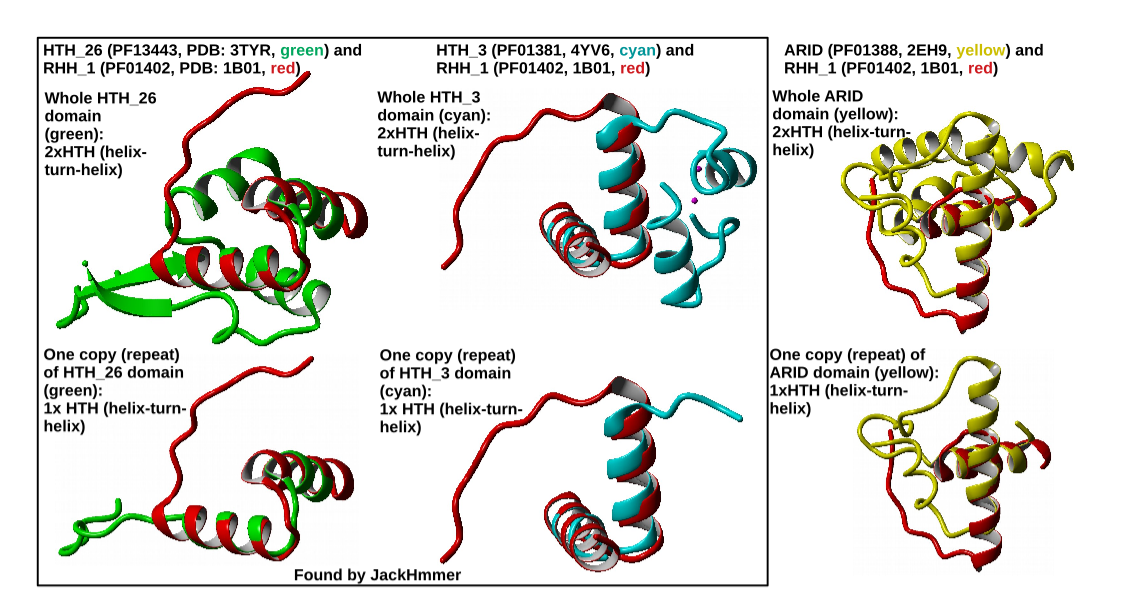
\includegraphics[width=0.8\textwidth]{superimpose_2_1}
\caption{Superimposition of RHH\_1 domain (Met\_repress CL0057) to HTH domains (HTH CL0123)}
\end{figure}

\begin{figure}[H]
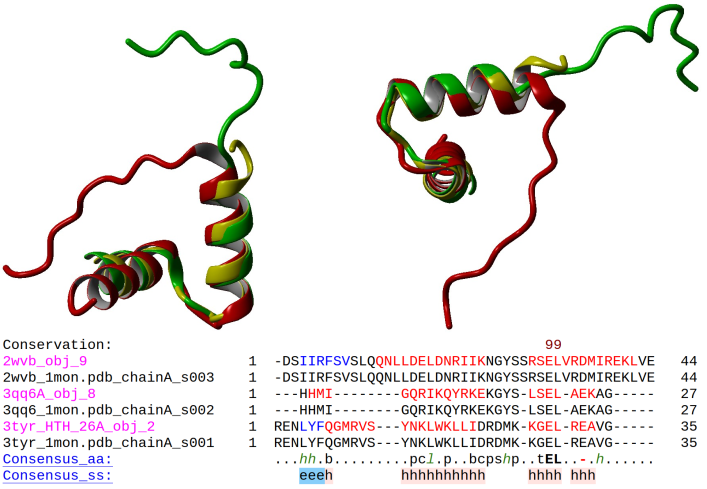
\includegraphics[width=\textwidth]{superimpose_1}
\caption{Superimposition and structural alignment (Promals3D) of RHH 1 structure (2WVB) and outgroups from clan CL0123
HTH 26 (3TYR), HTH 3 (3QQ6). Original file source: Outgroups\_HTH\_and\_RHH.}
\end{figure}

\begin{figure}[H]
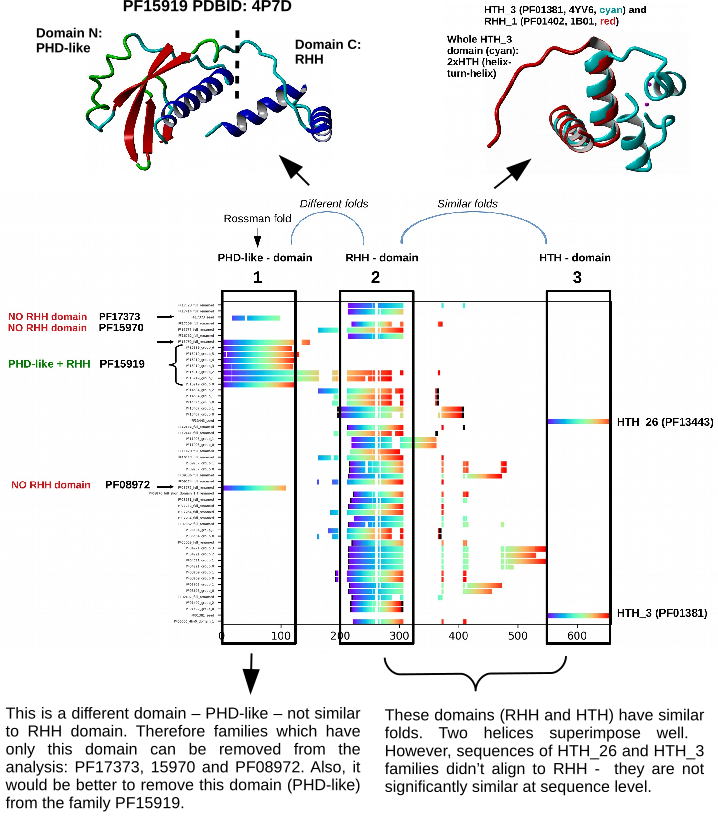
\includegraphics[width=\textwidth]{outgroups_1}
\end{figure}

        \subsection{Selected families and outgroups}
After further analysis correct outgoups were chosen.
    \begin{itemize}
        \item PF05261 - Tra\_M / DNA-binding - CL0548 (IHF-likeDNA-bdg)
        \item PF13443 - HTH\_26 - CL0123 (HTH)
        \item PF01381 - HTH\_3 - CL0123 (HTH)
    \end{itemize}

From clan CL0057 only families with RHH were picked.

Those files were the base for further analysis.

        




